
                \begin{figure}
                    \centering
                    \begin{tikzpicture}
                        \pgfplotsset{%
                            width=1\textwidth,
                            height=0.4\textheight
                        }
                        \begin{axis}[
                            xlabel={Runs since restart},
                            ylabel={Average dynamic energy (watt)},
                            ymin=0,ymax=70,
                        ]
                        
                            \addplot [mark=none, densely dashed, red]  coordinates {
                            (1, 0.03565424913569848)(2, 0.021178795117488047)(3, 0.020891514182504716)(4, 0.017436332622598767)(5, 0.01944345311675222)
                            };
                            \addlegendentry{WRK - IPG}
                            
                            \addplot [mark=none, densely dashed, blue]  coordinates {
                            (1, 0.06992167507263075)(2, 0.026254872202381527)(3, 0.018696399822635237)(4, 0.026544997056664552)(5, 0.01777578202292592)
                            };
                            \addlegendentry{WRK - LHM}
                            
                            \addplot [mark=none, densely dashed, cyan]  coordinates {
                            (1, 0.0)(2, 0.0)(3, 0.0)(4, 0.0)(5, 0.0)
                            };
                            \addlegendentry{WRK - CLAMP (win)}
                            
                        \end{axis}
                    \end{tikzpicture} 
                \caption{A graph illustrating the energy consumption of Dram for test case Fasta with regards to how long ago the DUT was restarted, experiment \#2, (with outliers)} \label{fig:Fasta_Dram_iteration_exp2}
                \end{figure}
                